\chapter{Preliminaries}

Before we can discuss variants of the BFGS method, and quasi-Newton methods in general, we introduce certain basic principles and aspects, which will be needed later, in this section. The theoretical concepts have been taken from \cite{BerkolaikoKuchment:2013} where they are discussed in more detail and more background information can be found.

\section{Metric Graphs}

We define a graph $\Gamma$ as an ordered pair $(\mathcal{V}, \mathcal{E})$, where $\mathcal{V} = \{v_i\}$ is a finite set of points, which we call vertices, and $\mathcal{E} = \{e_j\}$ is a set of segments connecting some of the vertices, which we call edges. In the following we will use the notation $E \coloneqq \left\lvert \mathcal{E} \right\rvert$ for the number of edges and $V \coloneqq \left\lvert \mathcal{V} \right\rvert$ for the number of vertices. \\
Each edge $e \in \mathcal{E}$ can be identified with a pair $(v, w)$ of vertices $v, w \in \mathcal{V}$, which it connects. A graph $\Gamma = (\mathcal{V}, \mathcal{E})$ is called directed graph, if each of its edges $e \in \mathcal{E}$ is assigned a direction, which means that each edge can only be followed in one direction. In this case, the order of the pair of vertices $(v, w)$ describing an directed edge $e$ is important, so that the set of directed edges $\mathcal{E}$ can be uniquely described as a set of ordered pairs $\mathcal{E} = \{e_i\}_{i = 1, \ldots, E} = \{(v^{o}_{i}, v^{t}_{i})\}_{i = 1, \ldots, E}$, where the first vertex $v^{o}_{i}$ is called the origin vertex and the second vertex $v^{t}_{i}$ is called the terminal vertex of the corresponding edge $e_i$. 

The origin and terminal points of a bond are specified via functions  and , i.e. a bond b begins at vertex  and ends at . We define the set of incoming bonds at a vertex v as the set of bonds satisfying t(b) = v. If o(b) = v, the bond b is called outgoing at vertex v.

A graph $\Gamma = (\mathcal{V}, \mathcal{E})$ is non-directed if each of its edges $e \in \mathcal{E}$ can be followed in both directions. In this case, the order of the two connected vertices describing an edge is unimportant, i.e. $e = (v, w) = (w, v)$, $v, w \in \mathcal{V}$. \\

\begin{figure}[H]
    \begin{subfigure}[b]{0.4\textwidth}
        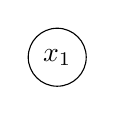
\begin{tikzpicture}[main/.style = {draw, circle}] 
            \node[main] (1) {$x_1$}; 
        \end{tikzpicture}
        \caption{Non-directed graph.}
        \label{fig:f1}
    \end{subfigure}
    \hfill
    \begin{subfigure}[b]{0.4\textwidth}
        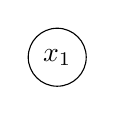
\begin{tikzpicture}[main/.style = {draw, circle}] 
            \node[main] (1) {$x_1$}; 
        \end{tikzpicture}
        \caption{Directed graph.}
        \label{fig:f2}
    \end{subfigure}
    \caption{Graphs.}
\end{figure}

Most frequently, in our considerations a non-directed graph will be considered as a digraph by assigning two bonds b and b with opposite directions to each edge e, as shown in Figure 2. We denote the resulting directed graph by 

% Graphik

The graph  satisfies the condition that at each vertex  v the numbers of incoming and outgoing bonds are equal: (the notation dv := dv/2 will be used in this situation). The set of bonds of  is symmetric in the sense that  if and only if there is another bond such that o(b) = t(b) and t(b) = o(b). The bond b is called the reversal of b. The operation of reversal is reflexive: b = b.
\\
A vertex $w \in \mathcal{V}$ is adjacent to a vertex $v \in \mathcal{V}$, denoted by $v \sim w$, if a suitable edge $e \in \mathcal{E}$ exists, so that $w$ can be reached from $v$ via this edge $e$. In the following we assume that a graph has no loops, which are edges that connect a vertex $v \in \mathcal{V}$ to itself, i.e. $v \sim v$, and no multi-edges, which are several equal edges between two vertices, i.e. $e_1, e_2 \in \mathcal{E}$ and $e_1 = e_2$. A graph $\Gamma = (\mathcal{V}, \mathcal{E})$ with $\mathcal{V} = \{v_i\}_{i = 1, \ldots, V}$ is fully specified by its $V \times V$ adjacency matrix $A^{\Gamma}$. The elements of the adjacency matrix are given by
\begin{equation}
    \label{adjacency matrix}
    A^{\Gamma}_{i, j}= \begin{cases} 1 & \text { if } v_i \sim v_j \\ 0 & \text { otherwise. } \end{cases}
\end{equation}
One sees immediately that the adjacency matrix of an undirected graph is symmetric, since a vertex $v \in \mathcal{V}$ is adjacent to another vertex $w \in \mathcal{V}$ exactly when the other way round is also true, i.e. $v \sim w \Leftrightarrow w \sim v$. \\
The degree $d_{v_i}$ of a vertex $v_i \in \mathcal{V}$ is the number of edges emanating from it, i.e. $d_{v_i} = \sum_{v_j \in \mathcal{V}} A_{i, j}$. All degrees are assumed to be finite. We will denote by $D^{\Gamma}$ the degree matrix of the graph, which is a diagonal $V \times V$ matrix with the entries
\begin{equation}
    \label{degree matrix}
    D^{\Gamma}_{i, j} = d_{v_i} \, \delta_{v_j, v_i}
\end{equation}
where $\delta_{v_j, v_i}$ is the Kronecker delta. \\

The number of incoming (respectively, outgoing) bonds at a vertex v is called incoming (resp.outgoing) degree of v and denoted  (resp. dov). Clearly, dov + div = dv.

A vertex is incident to an edge, denoted by $v \in e$, if the vertex $v \in \mathcal{V}$ is one of the two vertices the edge $e \in \mathcal{E}$ connects. We define for an undirected graph $\Gamma = (\mathcal{V}, \mathcal{E})$ with $\mathcal{V} = \{v_i\}_{i = 1, \ldots, V}$ and $\mathcal{E} = \{e_i\}_{i = 1, \ldots, E}$ the $V \times E$ incidence matrix $B^{\Gamma}$ by  
\begin{equation}
    \label{incidence matrix undirected}
    B^{\Gamma}_{i, j}= \begin{cases} 1 & \text { if } v_i \in e_j \\ 0 & \text { otherwise } \end{cases}
\end{equation}
and for a directed graph $\Gamma = (\mathcal{V}, \mathcal{E})$ with $\mathcal{V} = \{v_i\}_{i = 1, \ldots, V}$ and $\mathcal{E} = \{e_i\}_{i = 1, \ldots, E}$ we define the $V \times E$ incidence matrix $B^{\Gamma}$ by 
\begin{equation}
    \label{incidence matrix directed}
    B^{\Gamma}_{i, j}= \begin{cases} 1 & \text { if } e_j = (v_i, \cdot) \\ -1 & \text { if } e_j = (\cdot, v_i) \\ 0 & \text { if } v_i \notin e_j. \end{cases}
\end{equation}

% We also denote by $\mathcal{E}_v$ the set of all edges incident to the vertex $v$ (i.e., containing $v$). It is assumed that the degree (valence) dv = |Ev| of any vertex v is finite and positive. We hence exclude vertices with no edges coming in or going out.

So far we have considered graphs as discrete combinatorial objects. From now on we consider graphs as 1-dimensional complexes and the edges will be treated as 1-dimensional segments. If one considers graphs as 1D complexes, which we will often do, there exists a natural projection that maps the points x

%Grafik

Roughly speaking, we now imagine the edges $\mathcal{E}$ of a graph $\Gamma = (\mathcal{V}, \mathcal{E})$ not as abstract relations between the vertices $\mathcal{V}$, but rather as physical “wires” connecting them. For that we add a structure that equips $\Gamma$ with a topology and metric. 

\begin{definition}\label{metric graph}
    A graph $\Gamma = (\mathcal{V}, \mathcal{E})$ is said to be a metric graph, if each of its edges $e \in \mathcal{E}$ is assigned a positive length $l_e > 0$.
\end{definition}

%Having the length assigned, an edge e will be identified with a finite or infinite segment [0, le] of the real line with the natural coordinate xe along it. In most cases we will drop the subscript in the coordinate and call it x, which should not lead to any confusion. This enables one to interpret the graph Γ as a topological space (simplicial complex) that is the union of all edges where the ends corresponding to the same vertex are identified


\section{Drift-Diffusion Equations on Metric Graphs}
\label{ch1:sec2}

In this section, we introduce a model that uses a set of differential equations defined on the edges of a metric graph to represent the traffic flow in a road network. We want to approximate the solutions of these differential equations later in this thesis using different methods.  \\
We imagine a compact road network, where we mean a finite number of finitely long roads connected by a finite number of junctions. We note that in a realistic road network there also exist roads which simply start or end and we assume that these roads end or start in a junction to which no other roads are connected. Further there exist also one-way roads between two junctions in a realistic road network. To model such a compact road network, we identify it with a compact directed metric graph $\Gamma = (\mathcal{V}, \mathcal{E})$, where obviously the roads are identified by edges $e \in \mathcal{E}$ and the junctions by vertices $v \in \mathcal{V}$. The length $\ell_e > 0$ of each edge $e \in \mathcal{E}$ is either given by the length of the associated road or some other isometric representation of it. An example of such a compact road network is illustrated in \cref{fig8:f1} and the associated graph is illustrated in \cref{fig8:f2}. \\

\begin{figure}[H]
    \begin{center}
        \begin{subfigure}[b]{0.4\textwidth}
            \begin{center}
                \includegraphics[scale=0.45]{img/Kaßberg2.png}
            \end{center}
            \caption{Non-directed graph}
            \label{fig8:f1}
        \end{subfigure}
        \begin{subfigure}[b]{0.4\textwidth}
            \begin{center}
                \includegraphics[scale=0.2]{img/Kaßberg2-Darstellung.png}
            \end{center}
            \caption{Directed graph}
            \label{fig8:f2}
        \end{subfigure}
    \end{center}
    \caption{Two different types of graphs.}
\end{figure}

There exist several approaches to model the traffic flow on a road network. One of the most important approaches was presented in \cite{LighthillWhitham:1955}, and independently in \cite{Richards:1956}, in which the traffic flow is described by equations describing the flow of water. These fluid dynamics equations are a set of partial differential equations known as the Navier-Stokes equations, which express the conservation of mass, momentum, and energy. The basic idea of this approach is to look at large scales so to consider individual cars as small particles, a set of cars as mass, and their density as the main quantity to be considered, \cite[p.~1]{GaravelloPiccoli:2006}. The model in this thesis is inspired by the same idea. We also focus on the density of cars on an individual edge $e \in \mathcal{E}$ and we model it with a function $\rho_e \colon (0, T) \times [0, \ell_e] \to \mathbb{R}_{+}$. The value $\rho_e (t,x)$ describes the concentration of some quantity at the time $t \in (0, T)$ at the coordinate $x \in [0, \ell_e]$ on the edge $e \in \mathcal{E}$. It is reasonable to assume the conservation of the number of cars, which can be expressed by the following continuity equation for each individual edge $e \in \mathcal{E}$
\begin{equation}
    \label{continuity equation}
    \partial_t \rho_e (t,x) = - \partial_x J_e(t,x),
\end{equation}
where $J_e \colon (0,T) \times [0, \ell_e] \to \mathbb{R}$ is the flux of cars. \cref{continuity equation} expresses a relationship between the density of cars and the flux of cars by linking the temporal change of the density to the spatial change of its flux with the assumption of the conservation of the number of cars. Therefore, the conservation law given by \cref{continuity equation} describes the transport of a certain amount of cars. \\
Let the flux for the model in this thesis be given by 
\begin{equation} 
    \label{eq:flux} 
    J_e(t,x) \coloneqq - \varepsilon \partial_x \rho_e (t, x) + f(\rho_e(t, x)) \partial_x V_e(t, x).
\end{equation}
The flux is composed of two terms. The first term, $- \varepsilon \partial_x \rho_e (t, x)$, describes the transport by diffusion, which is given by Fick's first law, see \cite{Fick:1855}, where $\varepsilon > 0$ is the so-called diffusion coefficient. The second term, $f(\rho_e(t, x)) \partial_x V_e(t, x)$, describes the transport by flow or by drift, where $V_e \colon (0,T) \times [0, \ell_e] \to \mathbb{R}_{+}$ is a given potential, that may vary from edge to edge, the function $f \colon \mathbb{R}_{+} \to \mathbb{R}_{+}$ is called mobility and its simplest choice is the so-called linear transport $f(\rho_e) = \mathrm{v} \rho_e$ with $\mathrm{v}$ the average velocity of the cars. However, in many applications, the density $\rho_e (t,x)$ is not allowed to exceed a maximal value $\rho_{e, max}$, e.g. due to finite size effects. For the model in this thesis it is required that the mobility $f$ satisfies $f(0) = f(\rho_{e, max}) = 0$. If this value $\rho_{e, max}$ is scaled to one, a choice of $f$ that obeys $f(0) = f(1) = 0$, such as $f(\rho_e) = (1-\rho_e) \rho_e$, will ensure that solutions to \eqref{continuity equation} will satisfy this bound for all time. By choosing $f(\rho_e) = (1-\rho_e) \rho_e$, the average velocity of the cars $\mathrm{v}$ can be thought of as a linearly decreasing function depending on $\rho_e$, i.e. $\mathrm{v} = \mathrm{v}_{max} (1-\rho_e)$ with $\mathrm{v}_{max} > 0$. We follow this approach for the model in this thesis, but we set $\mathrm{v}_{max} = 1$. We note that with this choice of mobility $f$, it follows that all edges of the graph $\Gamma$ must be directed, because by defining the flux $J_e(t,x)$ via \cref{eq:flux} we consider first order derivatives in \cref{continuity equation} on the graph $\Gamma$ and for that one needs directions. We further note that the derivatives in $J_e(t,x)$ are taken into the outgoing direction. \\

Summarized, we have for the traffic flow in a compact road network a mathematical model, which is posed on a compact directed metric graph $\Gamma = (\mathcal{V}, \mathcal{E})$, where each edge $e \in \mathcal{E}$ is equipped with a length $\ell_e > 0$ and the following differential equation
\begin{equation} 
    \label{Drift-Diffusion-equation}
    \partial_t \rho_e (t,x) = \partial_x (\varepsilon \partial_x \rho_e (t,x) - f(\rho_e (t,x) ) \partial_x V_e (t,x)),
\end{equation}
where $\rho_e \colon (0, T) \times [0, \ell_e] \to [0, 1]$ is the objective function, $\varepsilon > 0$ is a constant, $V_e \colon (0,T) \times e \to \mathbb{R}_{+}$ is a given potential and $f \colon \mathbb{R}_{+} \to \mathbb{R}_{+}$ is a function, that satisfies $f(0) = f(1) = 0$. From now on, we refer to the differential equation given by \cref{Drift-Diffusion-equation} as drift-diffusion equation. \\
To make \cref{Drift-Diffusion-equation} a well-posed problem, we need to add initial-conditions as well as coupling conditions on the vertices. First we impose on each edge $e \in \mathcal{E}$ the following initial condition
\begin{equation}
    \label{eq:initial_conditions}
    \rho_e(0,x) = \rho_{e, 0}(x),
\end{equation}
where $\rho_{e, 0} \in L^2(e)$ returns the density on each point of the edge $e$ at the start time of the observation $t=0$. \\ 
In the following we denote the ordered pair of vertices connected by a directed edge $e \in \mathcal{E}$ by $(v^{\operatorname{o}}_e, v^{\operatorname{t}}_e) = e$ and for the vertex condition we define a normal vector $n_e$ to each edge $e = (v^{\operatorname{o}}_e, v^{\operatorname{t}}_e)$ via $n_e(v^{\operatorname{o}}_e) = -1$ and $n_e(v^{\operatorname{t}}_e) = 1$. \\
On the set of interior vertices $v \in \mathcal{V}_\mathcal{K} \subset \mathcal{V}$, which are vertices that are incident to at least one incoming edge and at least one outgoing edge (i.e. $\forall v \in \mathcal{V}_\mathcal{K} \; \exists \ e_1, e_2 \in \mathcal{E}$ such that $v^{\operatorname{t}}_{e_1} = v$ and $v^{\operatorname{o}}_{e_2} = v$), we apply homogeneous Kirchhoff-Neumann coupling conditions, i.e. on each $v \in \mathcal{V}_\mathcal{K}$ holds
\begin{equation}
    \label{eq:Kirchhoff_Neumann_condition}
    \sum_{e\in \mathcal{E}_v} J_e(t,v) n_e (v)=0,
\end{equation}
where $\mathcal{E}_v$ is the edge set incident to the vertex $v$. Additionally, we ask the solution of \cref{Drift-Diffusion-equation} to be continuous on the set of interior vertices $\mathcal{V}_\mathcal{K}$, i.e. 
\begin{equation}
    \label{continuous on vertices}
    \rho_e(v) = \rho_{e'}(v) \quad \text{ for all }v \in \mathcal{V}_\mathcal{K},\; e,\,e' \in \mathcal{E}_v.
\end{equation}
On the set of exterior vertices $v \in \mathcal{V}_\mathcal{D} \coloneqq \mathcal{V} \setminus \mathcal{V}_\mathcal{K}$, which are vertices to which either only incoming or only outgoing edges are incident (i.e. either $v^{\operatorname{t}}_{e} = v$ or $v^{\operatorname{o}}_{e} = v$ holds $\forall e \in \mathcal{E}_v$), the solution $\rho$ should fulfill the so-called flux boundary conditions
\begin{equation}
    \label{eq:Dirichlet_conditions}
    \sum_{e\in \mathcal{E}_v}J_e(t, v) n_e (v)=-\alpha_v(t) (1-\rho_v) + \beta_v(t) \rho_v,\ \text{for all}\ v \in \mathcal{V}_\mathcal{D}, e \in \mathcal{E}_v,
\end{equation}
where $\alpha_v \colon (0,T) \to \mathbb{R}_{+}$ describes the rate of influx of mass into the network and $\beta_v \colon (0,T) \to \mathbb{R}_{+}$, ${v \in \mathcal{V}_\mathcal{D}}$ describes the velocity of mass leaving the network at the exterior vertices $v \in \mathcal{V}_\mathcal{D}$. We note that this choice ensures that the bounds $0 \leq \rho_e \leq 1$ are preserved. In typical situations, exterior vertices are either of the influx- or of the outflux type, i.e. $\alpha_v(t) \beta_v(t) \equiv 0$ for all $v \in \mathcal{V}_\mathcal{D}$ and $t \in (0,T)$. \\
The Kirchhoff-Neumann conditions given by \cref{eq:Kirchhoff_Neumann_condition} are the natural vertex conditions for the differential equation given by \cref{Drift-Diffusion-equation}, since they ensure, on the one hand, that exactly as much mass flows into each interior vertex $v \in \mathcal{V}_{\mathcal{K}}$ as flows out of it and, on the other hand, together with the flux boundary conditions given by \cref{eq:Dirichlet_conditions} they ensure that mass enters or leaves the system only via the exterior vertices $\mathcal{V}_\mathcal{D}$ for which either $\alpha_v(t)$ or $\beta_v(t)$ is positive. \\

We note that through \cref{Drift-Diffusion-equation} we obtain the following differential operator defined on the metric graph $\Gamma$
\begin{equation} 
    \label{eq:Hamiltonian}
    \mathcal{H} [\rho_e] (t,x) \coloneqq \partial_t \rho_e (t,x)  - \partial_x (\varepsilon \partial_x \rho_e (t,x) + f(\rho_e (t,x) ) \partial_x V_e (t,x)),
\end{equation}
and together with the above mentioned initial and vertex conditions we obtain a triple which satisfies the definition of a quantum graph, see \cref{quantum graph}. Nevertheless, for the sake of simplicity, we will refer to it as drift-diffusion equations on a metric graph in the rest of this thesis. \\
Unfortunately, to the best of the author's knowledge, there is no constructive proof yet of any form of an analytical solution of the set of drift-diffusion equations given by \cref{Drift-Diffusion-equation} defined on a metric graph under the above mentioned initial and vertex conditions. Therefore it is a reasonable approach to approximate the solution, which results in the approximation problem that we will attempt to address in this thesis. The field of applied mathematics offers both well-known and new approaches to solve this approximation problem. In this paper we deal with (quite) new techniques, which will be introduced generally in the next section. 


%=
%\begin{theorem} 
    %Given initial data $\rho_0 \in L^2(\Gamma)$ s.t. $0 \le \rho_0 \le 1$ a.e. on $\mathcal{E}$, there exists a unique weak solution $\rho \in L^2(0,T; H^1(\Gamma)) \cap H^1(0,T; (H^1)^*(\Gamma))$ s.t.
	%\begin{align*}
		%\sum_{e \in \mathcal{E}} \left(\int_e  \partial_t \rho_e \varphi_e \;dx + \int_e \partial_x \rho_e\partial_x \varphi_e \;dx\right) + \sum_{v \in \mathcal{V}_D} (-\alpha_v(t) (1-\rho_v) + \beta_v(t) \rho_v)\varphi(v) = 0,
	%\end{align*}
	%for all test functions $\varphi \in H^1(\Gamma)$.
%\end{theorem}

%Kirchhoff: alles was in den Knoten reinfließt muss auch rausfließen
% Kirchhoff: We note that the derivative is taken into the outgoing direction.
%operator nicht selbstadjungiert

% Analytische Lösung nicht möglich

\section{Neural Networks as Function Approximators}
\label{ch1:sec3}

In this section we introduce artificial neural networks, usually called neural networks, which are computing systems inspired by the biological neural networks that constitute animal brains. 

In more practical terms neural networks are non-linear statistical data modeling or decision making tools. They can be used to model complex relationships between inputs and outputs or to find patterns in data. It has been shown that these systems can be used very well as classifiers as well as regressors or function approximators. \\
These neural networks are based on simplified models of biological neurons, which are special cells within the nervous system which transmit information to other nerve cells. Each of these artificial neurons receives data as input. These inputs of one neuron are modified by weights and summed. Finally, an activation function controls the amplitude of the output. The artificial neurons are connected to each other. A single neuron may be connected to many other neurons and the total number of neurons and connections in a network may be extensive. The connections of the biological neuron are modelled as weights, where a positive weight reflects an excitatory connection, while negative values mean inhibitory connections. Each connection, like the synapses in a biological brain, can transmit a signal to other neurons, where the signal is a real number. The other neurons connected to that neuron receive this real number as part of their input and repeat the process. However, artificial neural networks are more about an abstraction of that information processing, less about replicating biological neural networks and neurons. The first mathematical model for a single neuron, termed the perceptron, was described in \cite{Rosenblatt:1958} and is still in use today. 

We want to use perceptrons and the neural networks constructed from them to generate function values (output) that approximate the values of the solution to our differential equation from data (input) that will be the domain of our differential equation. \\
We now describe how a perceptron transforms a reel-valued input into a one-dimensional output, as illustrated in \cref{fig4}. Let there be $n$ input values $x_1, \ldots, x_n \in \mathbb{R}$, which can be understood as the entries of a vector $x \in \mathbb{R}^n$. First one forms a biased linear combination with the input values, i.e. 
\begin{equation*}
    a = \sum^{n}_{i=1} w_i x_i + b = w^{\mathrm{T}} x + b,
\end{equation*}
where $w_1, \ldots, w_n \in \mathbb{R}$ are called weights and $b \in \mathbb{R}$ is called bias. In general, these weights and the bias are learned through data. The weighted sum $a$ is called activation in the context of neural networks. Then an activation function $\sigma \colon \mathbb{R} \to \mathbb{R}$, which is non-linear, is applied to the weighted sum $a$, so that the output of the neuron becomes
\begin{equation*}
    z = \sigma(\sum^{n}_{i=1} w_i x_i + b) = \sigma(w^{\mathrm{T}} x + b) = \sigma(a).
\end{equation*}

\begin{figure}[H]
    \begin{center}
        \includegraphics[scale=0.3]{img/diagram-20220205_1.png}
    \end{center}
    \caption{Illustration of the perceptron model for a single neuron.}
    \label{fig4}
\end{figure}

The choice of activation function is determined by the nature of the input and the assumed distribution of the output. When the activation function is for example equal to the Heaviside step function, i.e.
\begin{equation*}
    \sigma(x) = \begin{cases} 1 & \text{if } x \geq 0, \\ 0 & \text{if } x < 0, \end{cases}
\end{equation*}
then the perceptron coincides with a linear support vector classifier, see \cite[Chapter~7]{Bishop:2006}. \\
The activation function can be any non-constant, non-linear function, but those generally used are monotone increasing, continuous, and at least piecewise smooth. At present, the most popular activation function is the rectified linear unit, abbreviated ReLu, \cref{ReLu}. In recent decades, smoother activation functions have been used, such as the sigmoid function, \cref{Sigmoid}, or the hyperbolic tangent function, \cref{TanH}, \cite{}.
\begin{align}
    \sigma(y) &=\max \{y, 0\} & & \text{ rectified linear unit (ReLU) } \label{ReLu} \\
    \sigma(y) &=\frac{1}{1+\exp (-y)} & & \text{ sigmoid } \label{Sigmoid} \\
    \sigma(y) &=\tanh (y)=\frac{\exp (y)-\exp (-y)}{\exp (y)+\exp (-y)} & & \text{ hyperbolic tangent } \label{TanH}
\end{align}
A single perceptron can already be understood as a neural network, but it still has many limitations. Above all, the dimension of the output is limited to $1$. If one wants to create a multi-dimensional output, one arranges several perceptrons in a layer by distributing the input to exactly as many perceptrons as one needs the dimension of the output. Suppose the input has dimension $n$ and the output should have dimension $m$. The weights of the $m$ neurons on that layer can be conveniently organized into a matrix a matrix $W \in \mathbb{R}^{m \times n}$, where each row corresponds to the $n$ weights of each perceptron, i.e. $w^{i} \in \mathbb{R}^n$ for all $i = 1, \ldots, m$. The biases of the $m$ perceptrons are represented as a vector $b \in \mathbb{R}^m$. The weighted sum of the input $x \in \mathbb{R}^n$ with the addition of a bias for each perceptron can be computed as  
\begin{equation*}
    a = W x + b \in \mathbb{R}^m,
\end{equation*}
which is often referred as propagation function. To simplify the notation, we define the activation function $\sigma \colon \mathbb{R} \to \mathbb{R}$ for vector-valued input values $a \in \mathbb{R}^m$ by applying it component-wise: 
\begin{equation*}
    \sigma \colon \mathbb{R}^{m} \ni a \mapsto \sigma(a):= \left(
        \begin{array}
            {c} \sigma \left( a_{1} \right) \\
            \vdots \\
            \sigma\left(a_{m}\right)
        \end{array}
        \right) \in \mathbb{R}^{m}.
\end{equation*}
Unfortunately, the ability of a single layer of perceptrons to model any reasonably complicated function is not very pronounced. This led to the idea of connecting several such layers of neurons one after the other, and utilizing the outputs from one layer of neurons as inputs to the neurons of the subsequent layer. From now on, we will refer to such a composition of layers of artificial neurons as a neural network. \\
We assume that we have $L \in \mathbb{N}$ layers of artificial neurons and we would like to connect them one after the other. Let us consider one layer of artificial neurons. We use n to denote the number of neurons in layer l. We denote the weight matrix by W and the bias by b. The matrix has n columns and m rows because it receives the output from the l-1 layer as input for the l layer and must generate nl linear combinations for the neurons in the l layer. The activation function can also depend on the layer, which is why we denote it with sigma. To simplify the notation, we introduce another layer to identify the input, which we will call the input layer. The number of neurons in this layer corresponds to the dimension of the input. This layer does not change the input and is the first layer of the network. The last layer of a neural network is called the output layer, whose number of neurons is equal to the desired dimension of the output. All other layers are called hidden layers. \\
A neural network now processes information as follows: The input from the input layer is passed to the first layer. 

The first layer has n neurons. Like the single layer shown above, it first calculates a matrix vector product with W and the input, adds a bias to it and applies an activation function to the activation in this first layer, so that the layer l=1 returns a vector z. This vector z is passed to layer 2 and the whole process is repeated until the last layer is reached.  


\begin{figure}[H]
    \begin{center}
        \includegraphics[scale=0.3]{img/diagram-20220206.png}
    \end{center}
    \caption{Illustration of an artificial neural network with $L=3$ layers.}
    \label{fig5}
\end{figure}

\begin{equation*}
    \mathbb{R}^{n^{(\ell-1)}} \ni \underbrace{x^{(\ell-1)}}_{\text {input of layer } \ell} \mapsto x^{(\ell)}:=\underbrace{\sigma^{(\ell)}\left(\left(W^{(\ell)}\right)^{\top} x^{(\ell-1)}+b^{(\ell)}\right)}_{\text {output of layer } \ell}=: F^{(\ell)}\left(x^{(\ell-1)}, W^{(\ell)}, b^{(\ell)}\right) \in \mathbb{R}^{n^{(\ell)}} .
\end{equation*}


\begin{equation*}
    \begin{aligned}
        y &=\sigma^{(3)}\left(\left(W^{(3)}\right)^{\top} \sigma^{(2)}\left(\left(W^{(2)}\right)^{\top} \sigma^{(1)}\left(\left(W^{(1)}\right)^{\top} x^{(0)}+b^{(1)}\right)+b^{(2)}\right)+b^{(3)}\right) \\
        &=F^{(3)}\left(F^{(2)}\left(F^{(1)}\left(x^{(0)}, W^{(1)}, b^{(1)}\right), W^{(2)}, b^{(2)}\right), W^{(3)}, b^{(3)}\right) \\
        &=: F\left(x^{(0)}, W^{(1)}, b^{(1)}, W^{(2)}, b^{(2)}, W^{(3)}, b^{(3)}\right) .
    \end{aligned}
\end{equation*}

They are obtained by organizing perceptrons in layers ` = 1, . . . , L and utilizing the outputs from one layer of neurons as inputs to the neurons of the subsequent layer,


the feed-forward neural network, also known as the multilayer perceptron,

The process of evaluating (5.7) can then be interpreted as a forward
propagation of information through the network.

In artificial neural networks, topology refers to the structure of the network. This generally means how many artificial neurons are located on how many layers and how they are connected to each other. Artificial neurons can be connected in many ways to form an artificial neural network. In many models, neurons are arranged in layers one behind the other; 

From a practical point of view, a network "learns" mainly by modifying the weights and biases of the neurons.


This generally means how many artificial neurons are on how many layers, and how they are connected to each other. Artificial neurons can be connected in many ways to form an artificial neural network. In many models, neurons are arranged in layers; a network with only one trainable neuron layer is called a single-layer network.

Using a graph, the neurons can be represented as vertices and their connections as edges. The inputs are sometimes also represented as nodes.

The rearmost layer of the network, whose neuron outputs are usually the only ones visible outside the network, is called the output layer. Layers before this are referred to as the hidden layer.

There are pure feedforward networks in which a layer is only ever connected to the next higher layer. In addition, there are networks in which connections are allowed in both directions. The appropriate network structure is usually found using the method of trial and error, which can be supported by evolutionary algorithms and error feedback.


Indeed,
it has been used very broadly to cover a wide range of different models, many of
which have been the subject of exaggerated claims regarding their biological plausibility. From the perspective of practical applications of pattern recognition, however, biological realism would impose entirely unnecessary constraints. Our focus in
this chapter is therefore on neural networks as efficient models for statistical pattern
recognition. In particular, we shall restrict our attention to the specific class of neural networks that have proven to be of greatest practical value, namely the multilayer
perceptron

Deep-learning methods are representation-learning methods with multiple levels of representation, obtained by composing simple but non-linear modules that each transform the representation at one level (starting with the raw input) into a representation at a higher, slightly more abstract level. With the composition of enough such transformations, very complex functions can be learned.

The most common form of machine learning, deep or not, is supervised learning.

The equations used for computing the forward pass in a neural net



The more complex the problem to be solved with the help of the neural network is, the more layers are needed. 

We compute an objective function that measures the error (or distance) between the output scores and the desired pattern of scores. The machine then modifies its internal adjustable parameters to reduce  this error. These adjustable parameters, often called weights, are real numbers that can be seen as ‘knobs’ that define the input–output function of the machine. In a typical deep-learning system, there may be hundreds of millions of these adjustable weights, and hundreds of millions of labelled examples with which to train the machine. To properly adjust the weight vector, the learning algorithm computes a gradient vector that, for each weight, indicates by what amount the error would increase or decrease if the weight were increased by a tiny amount. The weight vector is then adjusted in the opposite direction to the gradient vector. 

A deep-learning architecture is a multilayer stack of simple modules, all (or most) of which are subject to learning, and many of which compute non-linear input–output mappings. Each module in the stack transforms its input to increase both the selectivity and the invariance of the representation.

The backpropagation procedure to compute the gradient of an objective function with respect to the weights of a multilayer stack of modules is nothing more than a practical application of the chain rule for derivatives. The key insight is that the derivative (or gradient) of the objective with respect to the input of a module can be computed by working backwards from the gradient with respect to the output of that module

Many applications of deep learning use feedforward neural network architectures (Fig. 1), which learn to map a fixed-size input (for example, an image) to a fixed-size output (for example, a probability for each of several categories). To go from one layer to the next, a set of units compute a weighted sum of their inputs from the previous layer and pass the result through a non-linear function. At present, the most popular non-linear function is the rectified linear unit (ReLU), which is simply the half-wave rectifier. In past decades, neural nets used smoother non-linearities, such as , but the ReLU typically learns much faster in networks with many layers, allowing training of a deep supervised network without unsupervised pre-training28. Units that are not in the input or output layer are conventionally called hidden units. The hidden layers can be seen as distorting the input in a non-linear way so that categories become linearly separable by the last layer 



Perceptron
Activation Function
One layer
Neural Network
FNN
%ResNet
Machine Learning, Training 
Supervised Learning
Unsupervised Learning
Gradient Based optimization
Backpropagation 
Honrik 
\section{Physics-Informed Neural Networks}
\label{ch1:sec4}

In this section we describe physics-informed neural networks, abbreviated by PINNs, which  were introduced in \cite{RaissiPerdikarisKarniadakisPart1:2017} and are neural networks that are trained to solve supervised learning tasks while respecting any given law of physics described by general non-linear partial differential equations. PINNs enable the solution of a wide range of problems in computational science, represent a pioneering technology leading to the development of new classes of numerical solution methods for PDEs, and can be considered as a mesh-free alternative to traditional approaches and as a novel data-driven approach to model inversion and system identification \cite[p.~3]{RaissiPerdikarisKarniadakis:2019}. \\
Most of the physical laws that govern the dynamics of a system can be described by partial differential equations. For example, the Navier-Stokes equations are a set of partial differential equations derived from the conservation laws that describe the physics of many phenomena of scientific and engineering interest. They can be used to model the weather, ocean currents, water flow in a pipe and air flow around a wing. However, these equations cannot be solved exactly and therefore numerical methods must be used such as a finite volume method, where these equations must be solved while accounting for prior assumptions, linearization, and adequate time and space discretization. \\
As discussed in the previous section, machine learning methods with deep neural networks offer a promising way to approximate any map, therefore it is only logical to use them also for the approximation of the solution of differential equations. If one follows the classical approach, in which one trains a network purely by feeding it with data obtained, for example, from empirical tests of the underlying system, two problems arise. At first, when analysing complex physical, biological or technical systems, the cost of data acquisition is often prohibitive and one is faced with the challenge of drawing conclusions and making decisions based on incomplete information. For the often resulting small amount of data, most of the modern machine learning methods are not robust enough and offer no convergence guarantee, which is why the task of training a network with a few high-dimensional input and output values seems naive. Second, neural networks generally do not in general take into account the physical properties underlying the system generated from the physical law, and the degree of approximation accuracy they provide still depends heavily on a careful specification of the problem geometry and the initial and boundary conditions. Without this prior information, the solution is not unique and may lose physical correctness. Exactly this prior information, such as the principal physical laws governing the time-dependent dynamics of a system, or some empirically validated rules or other expertise, can act as a control agent that restricts the space of admissible solutions to a manageable size, which leads to the idea of a physics-informed neural network. This type of neural networks uses the governing physical equations in training, i.e. PINNs are designed to be trained to satisfy both the given training data and the given equations. In turn, encoding such structured information in a learning algorithm leads to an increase in the information content of the data which the algorithm encounters, so that it can move quickly towards the correct solution and generalise well, even when only a few training examples are available. Therefore, with some knowledge of the physical properties of the problem and some form of training data, PINNs can be used to find an optimal solution with high accuracy \cite{RaissiPerdikarisKarniadakisPart1:2017}. Moreover, PINNs can be used for data-driven discovery of partial differential equations or system identification, which is concerned with finding parameters that best describe the observed data of a test of a system. However, this is not relevant for this work and will therefore not be described. \\



If one follows the classical approach, in which one trains a network purely by feeding it with data obtained, for example, from empirical tests of the underlying system, two problems arise. 


a new class of data-efficient universal function approximators that naturally encode any underlying physical laws as prior information.



Depending on the nature and arrangement of the available data, we devise two distinct classes of algorithms, namely continuous time and discrete time models. The resulting neural networks form a new class of data-efficient universal function approximators that naturally encode any underlying physical laws as prior information

However, more often than not, in the course of analysing complex physical, biological or engineering systems, the cost of data acquisition is prohibitive, and we are inevitably faced with the challenge of drawing conclusions and making decisions under partial information.

At first sight, the task of training a deep learning algorithm to accurately identify a non-linear map from a few – potentially very high-dimensional – input and output data pairs seems at best naive. Coming to our rescue, for many cases pertaining to the modelling of physical and biological systems, there a exist a vast amount of prior knowledge that is currently not being utilized in modern machine learning practice. Let it be the principled physical laws that govern the time-dependent dynamics of a system, or some empirical validated rules or other domain expertise, this prior information can act as a regularization agent that constrains the space of admissible solutions to a manageable size. In return, encoding such structured information into a learning algorithm results in amplifying the information content of the data that the algorithm sees, enabling it to quickly steer itself towards the right solution and generalize well even when only a few training examples are available.



In this work we take a different approach by employing deep neural networks and leverage their well known capability as universal function approximators. In this setting, we can directly tackle non-linear problems without the need for committing to any prior assumptions, linearization, or local time-stepping. We exploit recent developments in automatic differentiation – one of the most useful but perhaps underused techniques in scientific computing – to differentiate neural networks with respect to their input coordinates and model parameters to obtain physics informed neural networks. 

This simple yet powerful construction allows us to tackle a wide range of problems in computational science and introduces a potentially disruptive technology leading to the development of new data-efficient and physics-informed learning machines, new classes of numerical solvers for partial differential equations, as well as new data-driven approaches for model inversion and systems identification

Given noisy measurements of the system, we are interested in the solution of two distinct problems. The first problem is that of predictive inference, filtering and smoothing, or data driven solutions of partial differential equations which states: given fixed model parameters  what can be said about the unknown hidden state of the system?



Therefore, a key property of physics-informed neural networks is that they can be effectively trained using small data sets; a setting often encountered in the study of physical systems for which the cost of data acquisition may be prohibitive

Automatic differentiation in general, and the back-propagation algorithm in particular, is currently the dominant approach for training deep models by taking their derivatives with respect to the parameters (e.g., weights and biases) of the models. Here, we use the exact same automatic differentiation techniques, employed by the deep learning community, to physics-inform neural networks by taking their derivatives with respect to their input coordinates (i.e., space and time) where the physics is described by partial differential equations.

Throughout this work we have been using relatively simple deep feed-forward neural networks architectures with hyperbolic tangent activation functions and no additional regularization

Burgers equation